% ------------------------------------------------------------------------------
% TYPO3 CMS 7.2 - What's New - Chapter "Introduction" (English Version)
%
% @author	Michael Schams <schams.net>
% @license	Creative Commons BY-NC-SA 3.0
% @link		http://typo3.org/download/release-notes/whats-new/
% @language	English
% ------------------------------------------------------------------------------
% LTXE-CHAPTER-UID:		16517900-07a67f43-fe9f3e35-7e924788
% LTXE-CHAPTER-NAME:	Introduction
% ------------------------------------------------------------------------------

\section{Introducción}
\begin{frame}[fragile]
	\frametitle{Introducción}

	\begin{center}\huge{Introducción}\end{center}
	\begin{center}\huge{\color{typo3darkgrey}\textbf{Los Hechos}}\end{center}

\end{frame}

% ------------------------------------------------------------------------------
% LTXE-SLIDE-START
% LTXE-SLIDE-UID:		22a897f8-73c1a0bd-fea4e9c4-cc112688
% LTXE-SLIDE-ORIGIN:	6d5e9f3e-f9d9677e-43d7d497-e80ba9ef English
% LTXE-SLIDE-TITLE:		TYPO3 CMS 7.2 - The Facts
% ------------------------------------------------------------------------------
\begin{frame}[fragile]
	\frametitle{Introducción}
	\framesubtitle{TYPO3 CMS 7.2 - Los Hechos}

	\begin{itemize}
		\item Fecha de lanzamiento: 28 de abril 2015
		\item Tipo de lanzamiento: "Lanzamiento Sprint"
		\item Visión: Adoptar, Innovar, Lanzar
		\item Foco principal: Frontend
	\end{itemize}

	\begin{figure}
		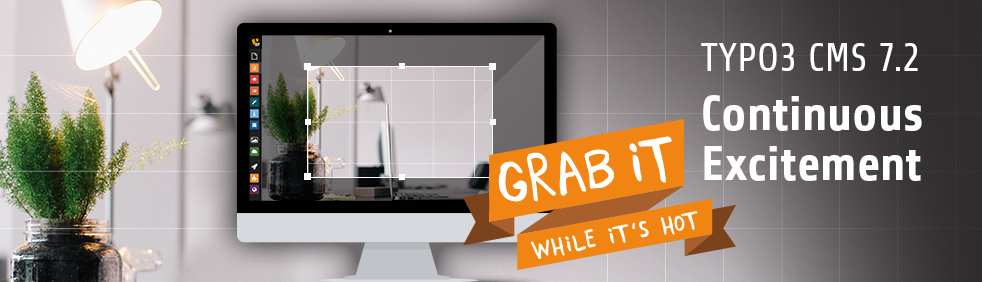
\includegraphics[width=0.95\linewidth]{Introduction/typo3cms72-teaser.png}
	\end{figure}

\end{frame}

% ------------------------------------------------------------------------------
% LTXE-SLIDE-START
% LTXE-SLIDE-UID:		4c15b5ca-e8dae825-9516251c-ace49b7c
% LTXE-SLIDE-ORIGIN:	759c3860-d5061f6e-2bb0009f-6ea130c8 English
% LTXE-SLIDE-TITLE:		System Requirements
% ------------------------------------------------------------------------------
\begin{frame}[fragile]
	\frametitle{Introducción}
	\framesubtitle{Requisitos del Sistema}

	\begin{itemize}
		\item PHP*:\tabto{3.4cm}v5.5.0 - v5.6.x
		\item MySQL:\tabto{3.4cm}v5.5.x - v5.6.x (modo no estricto)
		\item Espacio de disco:\tabto{3.4cm}min 200 MB
		\item Ajustes de PHP:

			\begin{itemize}
				\item memory\_limit >= 128M
				\item max\_execution\_time >= 240s
				\item opción de compilación \texttt{--disable-ipv6} \underline{no} debe ser usada
			\end{itemize}

		\item Backend requiere IE >= 9 o cualquier otro navegador moderno

	\end{itemize}

	\vspace{1cm}
	*) Detalles adicionales: \href{http://typo3.org/news/article/php-minimum-requirements-for-typo3-cms-7/}{Requisitos Mínimos de PHP para TYPO3 CMS 7}

\end{frame}

% ------------------------------------------------------------------------------
% LTXE-SLIDE-START
% LTXE-SLIDE-UID:		acbd1f26-b751df17-c8c041b9-9f350382
% LTXE-SLIDE-ORIGIN:	70c77c41-e2b83d82-2f182996-98061070 English
% LTXE-SLIDE-TITLE:		Development And Release Timeline
% ------------------------------------------------------------------------------
\begin{frame}[fragile]
	\frametitle{Introducción}
	\framesubtitle{Línea de tiempo de Desarrollo y Lanzamiento}

	\begin{figure}
		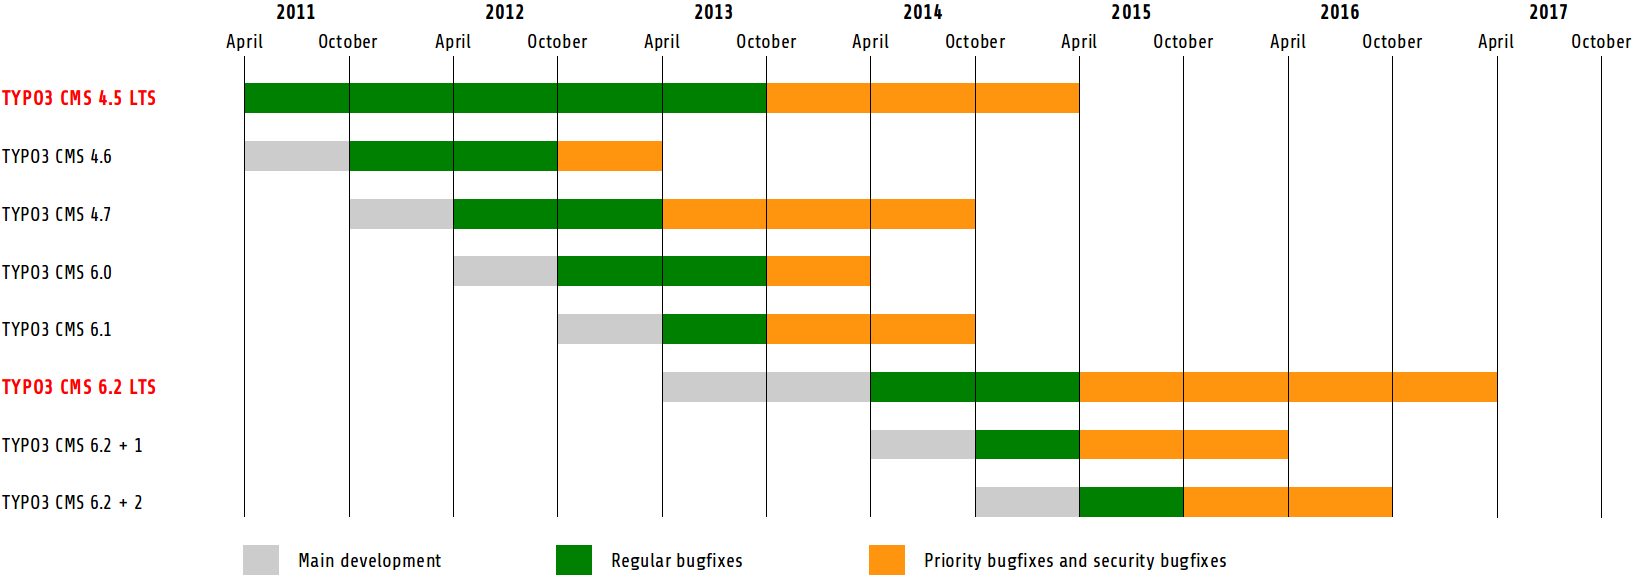
\includegraphics[width=0.90\linewidth]{Introduction/ReleaseAgenda.png}
	\end{figure}

\end{frame}

% ------------------------------------------------------------------------------
% LTXE-SLIDE-START
% LTXE-SLIDE-UID:		46139b2d-d3924726-87cc0124-521fa600
% LTXE-SLIDE-ORIGIN:	b55d3fe9-76807061-d97f3fee-7db1f190 English
% LTXE-SLIDE-TITLE:		TYPO3 CMS Roadmap
% ------------------------------------------------------------------------------
\begin{frame}[fragile]
	\frametitle{Introducción}
	\framesubtitle{Línea de lanzamiento de TYPO3 CMS}

	Fechas de lanzamiento estimadas y sus enfoques principales:

	\begin{itemize}
		\item v7.0 \tabto{1.0cm}02/Dic/2014\tabto{3.4cm}Revisión de Backend Vol 1
		\item v7.1 \tabto{1.0cm}24/Feb/2015\tabto{3.4cm}Optimización \& Limpieza del núcleo

		\item
			\begingroup
				\color{typo3orange}
					v7.2 \tabto{1.0cm}28/Abr/2015\tabto{3.4cm}Frontend
			\endgroup

		\item v7.3 \tabto{1.0cm}09/Jun/2015\tabto{3.4cm}Ecosistema de Paquete, Composer\newline
			\tabto{3.4cm}y Manejo de Extensiones
		\item v7.4 \tabto{1.0cm}04/Ago/2015\tabto{3.4cm}Revisión de Backend Vol 2
		\item v7.5 \tabto{1.0cm}29/Sep/2015\tabto{3.4cm}\textit{(por determinar...)}
		\item v7.6 \tabto{1.0cm}xx/xxx/2015\tabto{3.4cm}\textbf{TYPO3 CMS 7 LTS} (Soporte a Largo Plazo)
	\end{itemize}

	\smaller
		\url{https://typo3.org/typo3-cms/roadmap/}\newline
		\url{http://typo3.org/news/article/embrace-and-innovate-typo3-cms-7/}
	\normalsize

\end{frame}

% ------------------------------------------------------------------------------
% LTXE-SLIDE-START
% LTXE-SLIDE-UID:		d2044e00-40f7d3fe-6aa43f9e-48d81da6
% LTXE-SLIDE-ORIGIN:	b0c28f26-c3ca2e99-195954a8-ed76f9d4 English
% LTXE-SLIDE-TITLE:		Installation
% ------------------------------------------------------------------------------
\begin{frame}[fragile]
	\frametitle{Introducción}
	\framesubtitle{Instalación}

	\begin{itemize}
		\item Procedimiento de instalación oficial bajo Linux/Mac OS X\newline
			(DocumentRoot por ejemplo \texttt{/var/www/site/htdocs}):
		\begin{lstlisting}
			$ cd /var/www/site
			$ wget --content-disposition get.typo3.org/7.2
			$ tar xzf typo3_src-7.2.0.tar.gz
			$ cd htdocs
			$ ln -s ../typo3_src-7.2.0 typo3_src
			$ ln -s typo3_src/index.php
			$ ln -s typo3_src/typo3
			$ touch FIRST_INSTALL
		\end{lstlisting}

		\item Enlaces simbólicos bajo Microsoft Windows:

			\begin{itemize}
				\item Use \texttt{junction} en Windows XP/2000
				\item Use \texttt{mlink} en Windows Vista y Windows 7
			\end{itemize}

	\end{itemize}
\end{frame}

% ------------------------------------------------------------------------------
% LTXE-SLIDE-START
% LTXE-SLIDE-UID:		c0ea1a37-61671868-1dd8614d-d41361a1
% LTXE-SLIDE-ORIGIN:	48136734-ae508d23-bce5811d-667f8908 English
% LTXE-SLIDE-TITLE:		Upgrade to TYPO3 CMS 7
% ------------------------------------------------------------------------------
\begin{frame}[fragile]
	\frametitle{Introducción}
	\framesubtitle{Actualización a TYPO3 CMS 7.x}

	\begin{itemize}
		\item Actualizaciones sólo posibles desde TYPO3 CMS 6.2 LTS
		\item TYPO3 CMS < 6.2 deberá ser actualizado a TYPO3 CMS 6.2 LTS primero
	\end{itemize}

	\begin{itemize}

		\item Instrucciones de actualización:\newline
			\smaller\url{http://wiki.typo3.org/Upgrade#Upgrading_to_7.2}\normalsize
		\item Guía oficial de TYPO3 "Instalación y Actualización de TYPO3":
			\smaller\url{http://docs.typo3.org/typo3cms/InstallationGuide}\normalsize
		\item Enfoque general:
			\begin{itemize}
				\item Comprobar requisitos mínimos del sistema \small(PHP, MySQL, etc.)
				\item Revisar \textbf{deprecation\_*.log} en instancia antigua de TYPO3
				\item Actualizar todas las extensiones a las últimas versiones
				\item Desplegar fuentes nuevas y ejecutar:\newline
					Herramienta de Instalación \textrightarrow Asistente de Actualización
				\item Revisar el módulo de inicio para usuarios backend  (opcionalmente)
			\end{itemize}
	\end{itemize}

\end{frame}

% ------------------------------------------------------------------------------
